\documentclass{article}
\usepackage[utf8]{inputenc}
\usepackage[margin=1in]{geometry}
\usepackage{amsmath, amsfonts}
\usepackage{fancyhdr}
\usepackage{multicol}
\usepackage{graphicx}
\usepackage{amsthm}
\usepackage{pgfplotstable}
\usepackage{longtable}
\graphicspath{ {images/} }
\pagestyle{empty}
\fancyhf{}
\cfoot{\thepage}

\newtheorem*{lemma}{Lemma}
\newcommand{\twonorm}[1]{\| #1 \|_2}
\newcommand{\rdim}[2]{\mathbb{R}^{#1 \times #2}}
\newcommand{\R}{\mathbb{R}}
\lhead{CSCD37: Assignment \#1 }
\rhead{
Poon, Keegan\\
poonkeeg\\
1002423727}
\pagenumbering{gobble}
\renewcommand{\headrulewidth}{0pt}
\begin{document}

\thispagestyle{fancy}
\begin{enumerate}
  \item Consider the overdetermined linear system:
  \[ Ax = b,\: a \in \rdim{m}{n}, \; b \in \mathbb{R}^m,\: x \in \mathbb{R}^n, \: m > n.\]
  In lecture we proved that the best least-squares solution $x^*$ which minimizes $\twonorm{Ax-b}$ satisfies the normal equations $A^TAx=A^Tb$. Alternatively, we could proceed to find $x*$ as follows: Let
  \[ S(x) = \twonorm{Ax - b}^2 \]
  be a function of the $n$ variables $x_1,x_2,\dots,x_n$. A well-known result in calculus states that a necessary condition for $S$ to have a minimum at $x^*$ is that $x^*$ satisfies the system of equations
  \[ \frac{\partial S}{\partial x_i} = 0, \: i = 1,2,\dots,n.\]
  Show that this system is exactly the normal equations.
  
  What does the partial derivatives system look like? First, need to break down $Ax - b$.
  {
  \everymath{\displaystyle}
  \begin{align*}  
    Ax-b &= 
    \begin{bmatrix}
        a_{1,1} & a_{1,2} & \cdots & a_{1,n} \\
        a_{2,1} & a_{2,2} & \cdots & a_{2,n} \\
        \vdots  & \vdots  & \ddots & \vdots  \\
        a_{m,1} & a_{m,2} & \cdots & a_{m,n} 
    \end{bmatrix}
    \begin{bmatrix}
        x_{1} \\
        x_{2} \\
        \vdots \\
        x_{n}
    \end{bmatrix}
     - 
    \begin{bmatrix}
        b_{1} \\
        b_{2} \\
        \vdots \\
        b_{m}
    \end{bmatrix} \\
    &= 
    \begin{bmatrix}
        \sum_{i=1}^n a_{1,i} x_{i} \\
        \sum_{i=1}^n a_{2,i} x_{i} \\
        \vdots \\
        \sum_{i=1}^n a_{n,i} x_{i} \\
    \end{bmatrix}
     - 
    \begin{bmatrix}
        b_{1} \\
        b_{2} \\
        \vdots \\
        b_{m}
    \end{bmatrix} 
    = 
    \begin{bmatrix}
        \sum_{i=1}^n a_{1,i} x_{i} - b_1 \\
        \sum_{i=1}^n a_{2,i} x_{i} - b_2\\
        \vdots \\
        \sum_{i=1}^n a_{m,i} x_{i} - b_m\\
    \end{bmatrix}
  \end{align*}
  Hence $S(x)$ is 
    \[  \Big(\sum_{i=1}^n a_{1,i} x_{i} - b_1 \Big)^2 +
        \Big(\sum_{i=1}^n a_{2,i} x_{i} - b_2 \Big)^2 +
        \dots \\
        +\Big(\sum_{i=1}^n a_{m,i} x_{i} - b_m  \Big)^2\]
  So for some arbitrary $x_k$, because the other $x_j$ are held constant, $\frac{\partial S}{\partial x_k} = 0$  will be:
    \[  2 \Big(\sum_{i=1}^n a_{1,i} x_{i} - b_1 \Big)a_{1,k} +
        2 \Big(\sum_{i=1}^n a_{2,i} x_{i} - b_2 \Big)a_{2,k} +
        \dots \\
        +2 \Big(\sum_{i=1}^n a_{m,i} x_{i} - b_m  \Big)a_{m,k} = 0 \]
    \[ =  \Big(\sum_{i=1}^n (a_{1,k} a_{1,i} x_{i}) - a_{1,k}b_1  \Big) +
         \Big(\sum_{i=1}^n (a_{2,k}a_{2,i} x_{i}) - a_{2,k}b_2  \Big) +
        \dots \\
        + \Big(\sum_{i=1}^n (a_{m,k}a_{m,i} x_{i}) - a_{m,k}b_m \Big) = 0 \]
    \[ =  \sum_{j=1}^m \Bigg[ \sum_{i=1}^n (a_{j,k}a_{j,i} x_{i}) - a_{j,k}b_j \Bigg] = 0 \]
  Comparing this to the normal equations, what does that look like?
  \begin{align*}  
    A^TAx &= 
    \begin{bmatrix}
        a_{1,1} & a_{2,1} & \cdots & a_{m,1} \\
        a_{1,2} & a_{2,2} & \cdots & a_{m,2} \\
        \vdots  & \vdots  & \ddots & \vdots  \\
        a_{1,n} & a_{2,n} & \cdots & a_{m,n} 
    \end{bmatrix}
    \begin{bmatrix}
        a_{1,1} & a_{1,2} & \cdots & a_{1,n} \\
        a_{2,1} & a_{2,2} & \cdots & a_{2,n} \\
        \vdots  & \vdots  & \ddots & \vdots  \\
        a_{m,1} & a_{m,2} & \cdots & a_{m,n} 
    \end{bmatrix}
    \begin{bmatrix}
        x_{1} \\
        x_{2} \\
        \vdots \\
        x_{n}
    \end{bmatrix} \\
    &=
    \begin{bmatrix}
        \sum_{i=1}^m a_{i,1} a_{i,1} & \sum_{i=1}^m a_{i,1} a_{i,2} & \cdots &\sum_{i=1}^m a_{i,1} a_{i,n} \\
        \sum_{i=1}^m a_{i,2} a_{i,1} & \sum_{i=1}^m a_{i,2} a_{i,2} & \cdots & \sum_{i=1}^m a_{i,2} a_{i,n} \\
        \vdots  & \vdots  & \ddots & \vdots  \\
        \sum_{i=1}^m a_{i,n} a_{i,1} & \sum_{i=1}^m a_{i,n} a_{i,2} & \cdots & \sum_{i=1}^m a_{i,n} a_{i,n} 
    \end{bmatrix}
    \begin{bmatrix}
        x_{1} \\
        x_{2} \\
        \vdots \\
        x_{n}
    \end{bmatrix} \\
    &=\begin{bmatrix}
        x_1 \sum_{i=1}^m a_{i,1} a_{i,1} + x_2 \sum_{i=1}^m a_{i,1} a_{i,2} + \dots + x_n \sum_{i=1}^m a_{i,1} a_{i,n} \\
        x_1 \sum_{i=1}^m a_{i,2} a_{i,1} + x_2 \sum_{i=1}^m a_{i,2} a_{i,2} + \dots + x_n \sum_{i=1}^m a_{i,2} a_{i,n} \\
        \vdots \\
        x_1 \sum_{i=1}^m a_{i,n} a_{i,1} + x_2 \sum_{i=1}^m a_{i,n} a_{i,2} + \dots + x_n \sum_{i=1}^m a_{i,n} a_{i,n} \\
    \end{bmatrix} \\
    &=\begin{bmatrix}
        \sum_{i=1}^m \Big[ (x_1 a_{i,1} a_{i,1}) + (x_2a_{i,1} a_{i,2}) + \dots + (x_n  a_{i,1} a_{i,n}) \Big] \\
        \sum_{i=1}^m \Big[ (x_1 a_{i,2} a_{i,1}) + (x_2a_{i,2} a_{i,2}) + \dots + (x_n  a_{i,2} a_{i,n}) \Big] \\
        \vdots \\
        \sum_{i=1}^m \Big[ (x_1 a_{i,n} a_{i,1}) + (x_2a_{i,n} a_{i,2}) + \dots + (x_n  a_{i,n} a_{i,n}) \Big] \\
    \end{bmatrix} \\
    &=\begin{bmatrix}
        \sum_{i=1}^m \Bigg[ \sum_{j=1}^n (a_{i,1}a_{i,j} x_{j}) \Bigg]\\
        \sum_{i=1}^m \Bigg[ \sum_{j=1}^n (a_{i,2}a_{i,j} x_{j}) \Bigg]\\
        \vdots \\
        \sum_{i=1}^m \Bigg[ \sum_{j=1}^n (a_{i,n}a_{i,j} x_{j}) \Bigg]\\
    \end{bmatrix}
    = \begin{bmatrix}
        \sum_{j=1}^m \Bigg[ \sum_{i=1}^n (a_{j,1}a_{j,i} x_{i}) \Bigg]\\
        \sum_{j=1}^m \Bigg[ \sum_{i=1}^n (a_{j,2}a_{j,i} x_{i}) \Bigg]\\
        \vdots \\
        \sum_{j=1}^m \Bigg[ \sum_{i=1}^n (a_{j,n}a_{j,i} x_{i}) \Bigg]\\
    \end{bmatrix}
    \end{align*}
    \begin{align*}
        A^Tb &= 
    \begin{bmatrix}
        a_{1,1} & a_{2,1} & \cdots & a_{m,1} \\
        a_{1,2} & a_{2,2} & \cdots & a_{m,2} \\
        \vdots  & \vdots  & \ddots & \vdots  \\
        a_{1,n} & a_{2,n} & \cdots & a_{m,n} 
    \end{bmatrix}
    \begin{bmatrix}
        b_{1} \\
        b_{2} \\
        \vdots \\
        b_{m}
    \end{bmatrix} = 
    \begin{bmatrix}
        \sum_{j=1}^m a_{j,1}b_j \\
        \sum_{j=1}^m a_{j,2}b_j \\
        \vdots \\
        \sum_{j=1}^m a_{j,m}b_j\\
    \end{bmatrix}
    \end{align*}
    Putting all this into one equation, $A^TAx = A^Tb \iff A^TAx - A^Tb = 0$
    So 
    \[A^TAx - A^Tb = 0\]
    \[ \begin{bmatrix}
        \sum_{j=1}^m \Bigg[ \sum_{i=1}^n (a_{j,1}a_{j,i} x_{i}) \Bigg]\\
        \sum_{j=1}^m \Bigg[ \sum_{i=1}^n (a_{j,2}a_{j,i} x_{i}) \Bigg]\\
        \vdots \\
        \sum_{j=1}^m \Bigg[ \sum_{i=1}^n (a_{j,n}a_{j,i} x_{i}) \Bigg]\\
    \end{bmatrix} - 
    \begin{bmatrix}
        \sum_{j=1}^m a_{j,1}b_j \\
        \sum_{j=1}^m a_{j,2}b_j \\
        \vdots \\
        \sum_{j=1}^m a_{j,m}b_j\\
    \end{bmatrix}
    = 0\]
    \[ \begin{bmatrix}
        \sum_{j=1}^m \Bigg[ \sum_{i=1}^n (a_{j,1}a_{j,i} x_{i}) - a_{j,1}b_j \Bigg]\\
        \sum_{j=1}^m \Bigg[ \sum_{i=1}^n (a_{j,2}a_{j,i} x_{i}) - a_{j,2}b_j \Bigg]\\
        \vdots \\
        \sum_{j=1}^m \Bigg[ \sum_{i=1}^n (a_{j,n}a_{j,i} x_{i}) - a_{j,m}b_j \Bigg]\\
    \end{bmatrix}
    = 0\]
    Which is equivalent to the arbitrary $x_k$ system shown above for $S(x)$ when expanded to $k \in [1,n]$
  }
  \newpage
  \item In CSCC37 we saw how to compute the $PA = LU$ factorization of $A \in \mathbb{R}^{n\times n}$. The algorithm involved pre-multiplying $A$ with $n-1$ permutation matrices $\mathcal{P}_i$ interleaved with $n-1$ Gauss transforms $\mathcal{L}_i$, where $\mathcal{P}_i$, $\mathcal{L}_i \in \mathbb{R}^{n\times n}$, $i= 1,\dots,n-1$. This transformation triangularizes $A$, producing the upper-triangular matrix $U \in \mathbb{R}^{n \times n}$. The unit-lower triangular matrix $L \in \mathbb{R}^{n \times n}$ is later computed by a sequence of algebraic manipulations on  $\mathcal{P}_i$, $\mathcal{L}_i $, $i = 1, \dots, n-1$.
  \begin{enumerate}
    \newcommand{\calP}{\mathcal{P}}
    \newcommand{\calL}{\mathcal{L}}
      \item Show how $A \in \mathbb{R}^{m \times n}$, $m>n$ can be triangularized in a similar fashion using permutation matrices and Gauss transforms. Clearly specify the dimension and purpose of each $\mathcal{P}_i$ and $\mathcal{L}_i$ required, and the number of $\mathcal{P}_i$ and $\mathcal{L}_i$ required.

      (\textbf{Note:} You \textit{do not} need to show how to compute the final $L$.)

        In this case of an overdetermined system, the $LU$ factorization has to be defined, as $L$ and $U$ are not both square. $L$ will be a square matrix as to be able to chain multiple multiplications together, but $U$ will be the reduced form of $A$ with its upper $n$ rows forming an upper triangular matrix and its lower rows being 0.
        
        Given $A \in \rdim{m}{n}, m > n$ we can use permutation matrices $\calP_i \in \rdim{m}{m}$ to place the largest (magnitude) element of each column to the current row that we are eliminating from, similar to the method for square matrices. This is done by swapping the row we wish to eliminate from, to the row with the largest element in that column for each column.
        
        Not only do the $\calP_i$ have to be $m \times m$, but so do $\calL_i$ to be able to multiply against the other $\calP_i$ and $\calL_i$. Each of these, again analogous to the square case, will be used to eliminated everything underneath the $k$th row for the $k$th column in the exact same way using the diagonal element times the negative inverse of each other element.
        
        Since there are only $n$ columns that need to be eliminated, we will need $n$ of both $\calP$ and $\calL$. Note that this is different from the square case, we need one more of each. This is the case because we are not finished after doing the second last column, there will still be elements below the diagonal since we have a rectangular matrix so one more of each is required to clear the column.
      
      \item Given that the $PA = LU$ factorization of $A \in \mathbb{R}^{m \times n}$ , $m > n$ exists, \textbf{either} show how to use the factorization to solve the least squares problem $\min_x \twonorm{Ax - b}$, \textbf{or} argue why the $PA = LU$ factorization \textbf{cannot} be used.

     $PA = LU$ will not work for minimizing the norm. If the reason for $QR$ factorization working is examined, we see that $\twonorm{QRx - b} = \twonorm{Q^T[QRx-b]}$ which leads to $\twonorm{Ax-b} = {Rx-\tilde{b}}$. However, in the case of $LU$ factorization, we cannot multiply the equation by an inverse of $L$ and expect the norm to stay the same, this only worked since $Q$ orthogonal. This means that reducing the equation to $Ux = \tilde{b}$ will change the norm, and thus have no bearing on the original equation, so solving $LUx = \tilde{b}$ does not minimize the 2 norm of the original equation.
      
      \item Given that the $PA = LU$ factorization of $A \in \mathbb{R}^{m \times n}$ , $m > n$ exists, \textbf{either} show how to use the factorization to solve the null space problem $\min_x \twonorm{Ax - b}$, \textbf{or} argue why the $PA = LU$ factorization \textbf{cannot} be used. (Recall that in the null space problem, $A \in \mathbb{R}^{m \times n}, m > n$ arises by transposing the original coefficient matrix in the undetermined system.)

      The factorization cannot be used since again, the orthogonality of $Q$ is essential in the solution. If we examine the proof for the validity of the $QR$ factorization, and re create it for $PA = LU$ we get, 
      \begin{align*}
        PA &= LU \\
        (PA)^T &= U^TL^T \\
        (PA)^T {L^{-1}}^T &= U^T \\
      \end{align*}
      and here we see that ${L^{-1}}^T$ is what is being multiplied by, but the transpose negates the structure of $L_1$ $L_2$ that was exploited in $QR$ since the inverse was simply transpose, we get $Q$ back again. This does not hold for $LU$ and gives us a bogus system that does not help for solving. 
  \end{enumerate}
  \newpage
  \item Consider the overdetermined linear system:
  \[ Ax = b,\: a \in \rdim{m}{n}, \; b \in \mathbb{R}^m,\: x \in \mathbb{R}^n, \: m > n.\]
  In general there is no exact solution to this system and the best we can do to solve the problem is minimize the norm of the residual $Ax -b$. In certain cases, though, there \textit{is} an exact solution and the norm of the residual is zero. State the conditions required for this to happen and give an example.
  
  For there to be an exact solution, we must have that $b$ is in the range of $A$, i.e. $b$ is a linear combination of the columns of $A$. If it isn't the case, then $Ax$ being a linear combination of said column vectors, will never be equal to $b$.

  For examples, take
  \[
      A = [a_1, a_2, a_3] = 
      \begin{bmatrix}
          1 & 4 & 1 \\
          2 & 3 & 1 \\
          3 & 2 & 1 \\
          4 & 1 & 2 \\
      \end{bmatrix}, \:
      b = \begin{bmatrix} 6\\ 6\\ 6\\ 8\\\end{bmatrix}
  \]
    Then, we can see that $b$ is a linear combination of the columns, given as $a_1 + a_2 + 2a_3$, giving a solution $x = [1, 1, 2]$. If $b$ was not in the range, (say $b = [6, 6, 6, 7]$) then it would be impossible to solve it, as it is not a linear combination.
  \newpage
  \item In lecture we proved that the Householder transformation
  \newcommand{\calQ}{\mathcal{Q}}
  \[ \calQ = I - 2 \frac{vv^T}{v^Tv} \]
  is both orthogonal and symmetric for any $v \not = 0$, and we \textit{claimed} that if we choose 
  \begin{equation}
      v = x - \twonorm{x}e_1
  \end{equation}
  we have
  \begin{equation}
      \calQ x = \Bigg[I - 2 \frac{vv^T}{v^Tv} \Bigg] x = \twonorm{x}e_1
  \end{equation}
  where $e_1$ is the first column of the identity matrix. We then used (2) to compute the \textit{QR}-factorization by embedding a sequence of similar transformations in the identity matrix.
  Prove that if we choose $v$ as in (1), (2) holds.
  {
  \everymath{\displaystyle}
  \[
  x = 
  \begin{bmatrix}
    x_1 \\
    x_2 \\
    \vdots \\
    x_n
  \end{bmatrix}
  , \: v = 
  \begin{bmatrix}
    x_1 - \twonorm{x} \\
    x_2 \\
    \vdots \\
    x_n
  \end{bmatrix}
  \]
  \begin{align*} v^Tv &= 
  \begin{bmatrix}
    x_1 - \twonorm{x} \\
    x_2 \\
    \vdots \\
    x_n
  \end{bmatrix}
  \begin{bmatrix}
    x_1 - \twonorm{x}, &
    x_2, &
    \cdots, &
    x_n
  \end{bmatrix} \\
 & =  (x_1 - \twonorm{x})^2 + x_2^2 + \cdots + x_n^2 \\
 & = \twonorm{x}^2 - 2x_1\twonorm{x} + \sum_{i=1}^{n}x_i^2 \\
 & = \sum_{i=1}^{n}x_i^2 - 2x_1\twonorm{x} + \sum_{i=1}^{n}x_i^2 \\
 & =  2\sum_{i=1}^{n}x_i^2 - 2x_1\twonorm{x}
  \end{align*}
  \begin{align*}
     vv^T &= 
    \begin{bmatrix}
        (x_1 - \twonorm{x})^2 & (x_1 - \twonorm{x})x_2 & \cdots & (x_1 - \twonorm{x})x_n \\
        (x_1 - \twonorm{x})x_2 & x_2^2 & \cdots & x_2x_n \\
        \vdots  & \vdots  & \ddots & \vdots  \\
        (x_1 - \twonorm{x})x_n & x_2x_n & \cdots & x_n^2 
    \end{bmatrix}
  \end{align*}
  \begin{align*}
      \calQ x &= \Bigg[I - 2 \frac{vv^T}{v^Tv} \Bigg] x \\
      &= 
      \begin{bmatrix}
        x_1 \\
        x_2 \\
        \vdots \\
        x_n
      \end{bmatrix}
     - \frac{2}{2\sum_{i=1}^{n}x_i^2 - 2x_1\twonorm{x}}
     \begin{bmatrix}
        (x_1 - \twonorm{x})^2x_1 + (x_1 - \twonorm{x})x_2^2 + \cdots + (x_1 - \twonorm{x})x_n^2 \\
        (x_1 - \twonorm{x})x_2x_1 + x_2^3 + \cdots + x_2x_n^2 \\
        \vdots \\
        (x_1 - \twonorm{x})x_nx_1 + x_2^2x_n + \cdots + x_n^3 
    \end{bmatrix} \\
      &= 
      \begin{bmatrix}
        x_1 \\
        x_2 \\
        \vdots \\
        x_n
      \end{bmatrix}
     - \frac{1}{\sum_{i=1}^{n}x_i^2 - x_1\twonorm{x}}
     \begin{bmatrix}
        (x_1 - \twonorm{x}) \Big[ (x_1 - \twonorm{x})x_1 + \sum_{i=2}^{n}x_i^2 \Big] \\
        x_2 \Big[ (x_1 - \twonorm{x})x_1 + \sum_{i=2}^{n}x_i^2 \Big]\\
        \vdots  \\
        x_n \Big[ (x_1 - \twonorm{x})x_1 + \sum_{i=2}^{n}x_i^2 \Big] 
    \end{bmatrix} \\
      &= 
      \begin{bmatrix}
        x_1 \\
        x_2 \\
        \vdots \\
        x_n
      \end{bmatrix}
     - \frac{1}{\sum_{i=1}^{n}x_i^2 - x_1\twonorm{x}}
     \begin{bmatrix}
        (x_1 - \twonorm{x}) \Big[  - x_1\twonorm{x} + \sum_{i=1}^{n}x_i^2 \Big] \\
        x_2 \Big[ - x_1\twonorm{x} + \sum_{i=1}^{n}x_i^2 \Big]\\
        \vdots  \\
        x_n \Big[ - x_1\twonorm{x} + \sum_{i=1}^{n}x_i^2 \Big]
    \end{bmatrix} \\
    &= 
    \begin{bmatrix}
        x_1 \\
        x_2 \\
        \vdots \\
        x_n
      \end{bmatrix}
      -
     \begin{bmatrix}
        x_1 - \twonorm{x} \\
        x_2 \\
        \vdots  \\
        x_n
    \end{bmatrix} = 
     \begin{bmatrix}
        \twonorm{x} \\
        0\\
        \vdots  \\
        0
    \end{bmatrix} \text{As wanted}
  \end{align*}
  }
  \newpage
  \item Consider the overdetermined linear system $Ax = b$ where
  \[ A = 
  \begin{bmatrix}
    3 & 0 \\
    4 & 5 \\
    0 & 4 \\
  \end{bmatrix}
  ,\: b = 
  \begin{bmatrix}
    1 \\
    2 \\
    3 \\
  \end{bmatrix}.
  \]
  \begin{enumerate}
      \item Compute the \textit{QR}-factorization of $A$ using Householder reflections. Show \textit{all} intermediate calculations. For example, the first reflection is given by 
      \[
        \calQ_1 = I - 2 \frac{vv^T}{v^Tv} , \: v = a_1 - \twonorm{a_1}e_1
      \]
      where $a_1$ is the first column of $A$. Verify that $Q = \calQ_1^T\calQ_2^T$ is orthogonal.
      
  {
  \everymath{\displaystyle}
      \begin{align*}
          v &= 
          \begin{bmatrix}
            3 \\
            4 \\
            0 \\
          \end{bmatrix}
          - \sqrt{3^2 + 4^2}
          \begin{bmatrix}
            1 \\
            0 \\
            0 \\
          \end{bmatrix}
          = 
          \begin{bmatrix}
            3 \\
            4 \\
            0 \\
          \end{bmatrix}
          - 
          \begin{bmatrix}
            5 \\
            0 \\
            0 \\
          \end{bmatrix}
          = 
          \begin{bmatrix}
            -2 \\
            4 \\
            0 \\
          \end{bmatrix}
      \end{align*}
      \begin{align*}
          v^Tv = (-2)^2 + 4^2 = 20
      \end{align*}
      \begin{align*}
          vv^T &= 
          \begin{bmatrix}
            -2 \\
            4 \\
            0 \\
          \end{bmatrix}
          \begin{bmatrix}
            -2 & 4 & 0 
          \end{bmatrix} 
          = 
          \begin{bmatrix}
            4 & -8 & 0 \\
            -8 & 16 & 0 \\
            0 & 0 & 0\\
          \end{bmatrix}
      \end{align*}
      \begin{align*}
        \calQ_1 &= I - 2 \frac{vv^T}{v^Tv} 
        = 
        \begin{bmatrix}
        1 & 0 & 0 \\
        0 & 1 & 0 \\
        0 & 0 & 1 \\
        \end{bmatrix} 
        -  \frac{1}{10}
        \begin{bmatrix}
            4 & -8 & 0 \\
            -8 & 16 & 0 \\
            0 & 0 & 0\\
        \end{bmatrix} 
          = 
        \begin{bmatrix}
            3/5 & 4/5 & 0 \\
            4/5 & -3/5 & 0 \\
            0 & 0 & 1\\
        \end{bmatrix} \\
      \end{align*}
      \begin{align*}
          \calQ_1 A = 
          \begin{bmatrix}
            3/5 & 4/5 & 0 \\
            4/5 & -3/5 & 0 \\
            0 & 0 & 1\\
        \end{bmatrix} 
        \begin{bmatrix}
            3 & 0 \\
            4 & 5 \\
            0 & 4 \\
        \end{bmatrix}
        = 
        \begin{bmatrix}
            5 & 4 \\
            0 & -3 \\
            0 & 4 \\
        \end{bmatrix}
      \end{align*}
      \begin{align*}
          a_2 = 
          \begin{bmatrix}
            -3 \\
            4
          \end{bmatrix} 
          , \:
          v' = a_2 - \twonorm{a_2}e_1
          =
          \begin{bmatrix}
            -3 \\
            4
          \end{bmatrix} 
          - \sqrt{ (-3)^2 + (4)^2}
          \begin{bmatrix}
          1 \\
          0
          \end{bmatrix}
          = 
          \begin{bmatrix}
            -8 \\
            4
          \end{bmatrix} 
      \end{align*}
      \begin{align*}
          v'^Tv' = (-8)^2 + 4^2 = 80 , \:
          v'v'^T = 
          \begin{bmatrix}
            -8 \\
            4
          \end{bmatrix}
          \begin{bmatrix}
            -8 & 4
          \end{bmatrix}
          =
          \begin{bmatrix}
            64 & -32 \\
            -32 & 16 \\
          \end{bmatrix}
      \end{align*}
      \begin{align*}
          \calQ_2 = I - 2 \frac{v'v'^T}{v'^Tv'} =
          \begin{bmatrix}
            1 & 0 \\
            0 & 1 \\
          \end{bmatrix}
          - \frac{1}{40}
          \begin{bmatrix}
            64 & -32 \\
            -32 & 16 \\
          \end{bmatrix} 
          =
          \begin{bmatrix}
            -3/5 & 4/5 \\
            4/5 & 3/5 \\
          \end{bmatrix}
      \end{align*}
      Expanded to $\rdim{3}{3}$, 
      \[\calQ_2 = \begin{bmatrix} 1 & 0 & 0 \\ 0 & -3/5 & 4/5 \\
           0 & 4/5 & 3/5 \\ \end{bmatrix}\]
      This means that
      \[Q =  \calQ_1^T \calQ_2^T  = 
      \begin{bmatrix}
        3/5 & 4/5 & 0 \\
        4/5 & -3/5 & 0 \\
        0 & 0 & 1\\
      \end{bmatrix}
      \begin{bmatrix} 
        1 & 0 & 0 \\ 
        0 & -3/5 & 4/5 \\
        0 & 4/5 & 3/5 \\
      \end{bmatrix} =
      \begin{bmatrix} 
        3/5 & -12/25 & 16/25 \\ 
        4/5 & 9/25 & -12/25 \\
        0 & 4/5 & 3/5 \\
      \end{bmatrix}\] 
      Also, $R = \calQ_2 \calQ_1 A $
      \[
        \begin{bmatrix} 
          1 & 0 & 0 \\ 
          0 & -3/5 & 4/5 \\
          0 & 4/5 & 3/5 \\
        \end{bmatrix}
        \calQ_2 \calQ_1 A = 
        \begin{bmatrix}
            5 & 4 \\
            0 & -3 \\
            0 & 4 \\
        \end{bmatrix}
        =
        \begin{bmatrix}
            5 & 4 \\
            0 & 5 \\
            0 & 0 \\
        \end{bmatrix}
      \]
      Verifying that $Q$ is orthogonal,
      \[ QQ^T = 
      \begin{bmatrix}
        3/5 & 4/5 & 0 \\
        4/5 & -3/5 & 0 \\
        0 & 0 & 1\\
      \end{bmatrix}
      \begin{bmatrix} 
        1 & 0 & 0 \\ 
        0 & -3/5 & 4/5 \\
        0 & 4/5 & 3/5 \\
      \end{bmatrix}
      \begin{bmatrix} 
        1 & 0 & 0 \\ 
        0 & -3/5 & 4/5 \\
        0 & 4/5 & 3/5 \\
      \end{bmatrix}
      \begin{bmatrix}
        3/5 & 4/5 & 0 \\
        4/5 & -3/5 & 0 \\
        0 & 0 & 1\\
      \end{bmatrix} \] 
      \[ = 
      \begin{bmatrix}
        3/5 & 4/5 & 0 \\
        4/5 & -3/5 & 0 \\
        0 & 0 & 1\\
      \end{bmatrix}
      \begin{bmatrix} 
        1 & 0 & 0 \\ 
        0 & 1 & 0 \\
        0 & 0 & 1 \\
      \end{bmatrix}
      \begin{bmatrix}
        3/5 & 4/5 & 0 \\
        4/5 & -3/5 & 0 \\
        0 & 0 & 1\\
      \end{bmatrix}
      = 
      \begin{bmatrix}
        3/5 & 4/5 & 0 \\
        4/5 & -3/5 & 0 \\
        0 & 0 & 1\\
      \end{bmatrix}
      \begin{bmatrix}
        3/5 & 4/5 & 0 \\
        4/5 & -3/5 & 0 \\
        0 & 0 & 1\\
      \end{bmatrix} \] 
      \[ \begin{bmatrix}
        1 & 0 & 0 \\
        0 & 1 & 0 \\
        0 & 0 & 1\\
      \end{bmatrix} \text{As wanted} 
      \] 
      }
      \item Use the \textit{QR}-factorization in (a) to solve the least squares problem $\min_x\twonorm{Ax-b}$.
      \begin{align*}
          Ax &= b\\
          QRx &= b\\
          Rx &= Q^Tb\\
      \end{align*}
      \begin{align*}
          Q^Tb = 
          \begin{bmatrix} 
            3/5 & 4/5 & 0 \\ 
            -12/25 & 9/25 & 4/5 \\
            16/25 & -12/25 & 3/5 \\
          \end{bmatrix}
          \begin{bmatrix}
            1 \\
            2 \\
            3 \\
          \end{bmatrix}
          = 
          \begin{bmatrix}
            11/5 \\
            66/25 \\
            37/25 \\
          \end{bmatrix}
          \implies
          \tilde{b}_1 =
          \begin{bmatrix}
            11/5 \\
            66/25 \\
          \end{bmatrix}
      \end{align*}
      \begin{align*}
          R = 
          \begin{bmatrix}
            5 & 4 \\
            0 & 5 \\
            0 & 0 \\
          \end{bmatrix}
          \implies 
          \mathcal{R}_1 =
          \begin{bmatrix}
              5 & 4 \\
              0 & 5 \\
          \end{bmatrix}
      \end{align*}
      \begin{align*}
          66/25 = 5x^*_2 &\implies x^*_2 = 66/125 \\
          11/5 = 5x^*_1 + 4x^*_2 &\implies 275/125 = 5x^*_1 + 264/125 \\
          &\implies 11/125 = 5x^*_1 \\
          &\implies x^*_1 = 11/625 \\
          &\implies x^* =
          \begin{bmatrix}
            11/625 \\
            66/125 \\
          \end{bmatrix}
      \end{align*}
  \end{enumerate}
  \newpage
  \item As can be seen from the figures, for sufficiently large $n$, the least squares method gives a very accurate polynomial approximation to the function, within the range of interpolation. The vast majority of points in the interpolation range have less than 1\% relative error, and the graphs when inspected visually converge very closely to the original functions. The only case when this isn't happening is for the degree 2 parabola being used for log $x$ when approaching one, the relative error grows largely. This is likely due however, to the not having a high enough degree to sufficiently estimate, and the fact that log $x$ approaches 0, so any error will be magnified.
  
  \pgfplotstableset{
begin table=\begin{longtable},
end table=\end{longtable},
}
  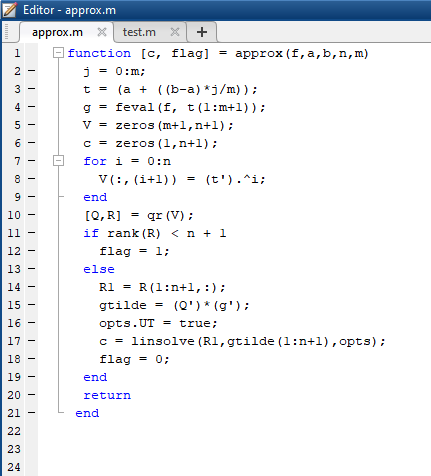
\includegraphics[width=\textwidth]{approx}
  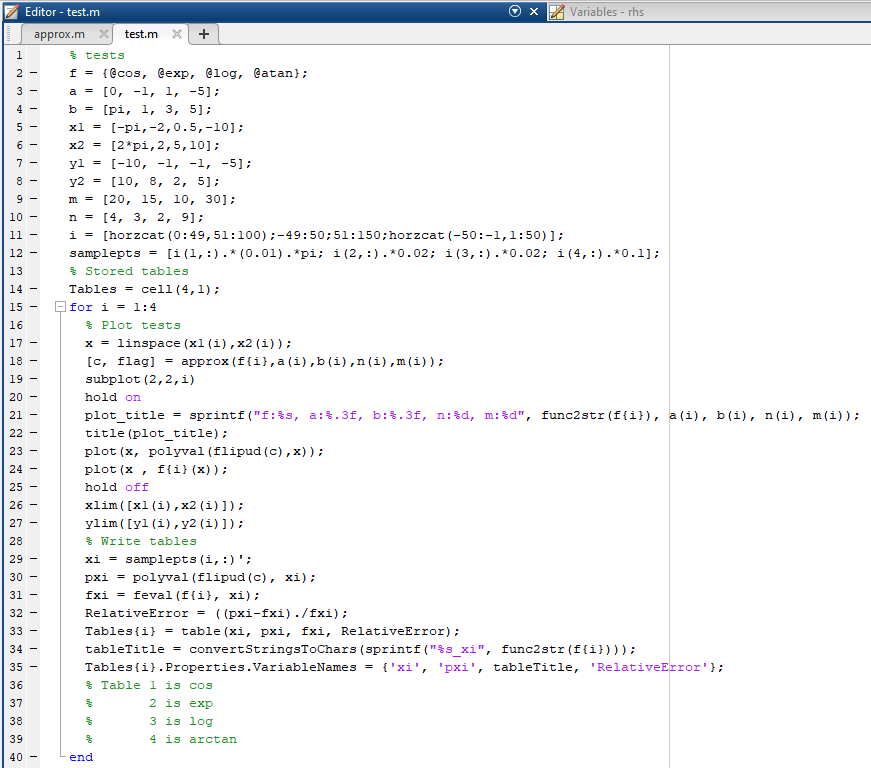
\includegraphics[width=\textwidth]{test}
  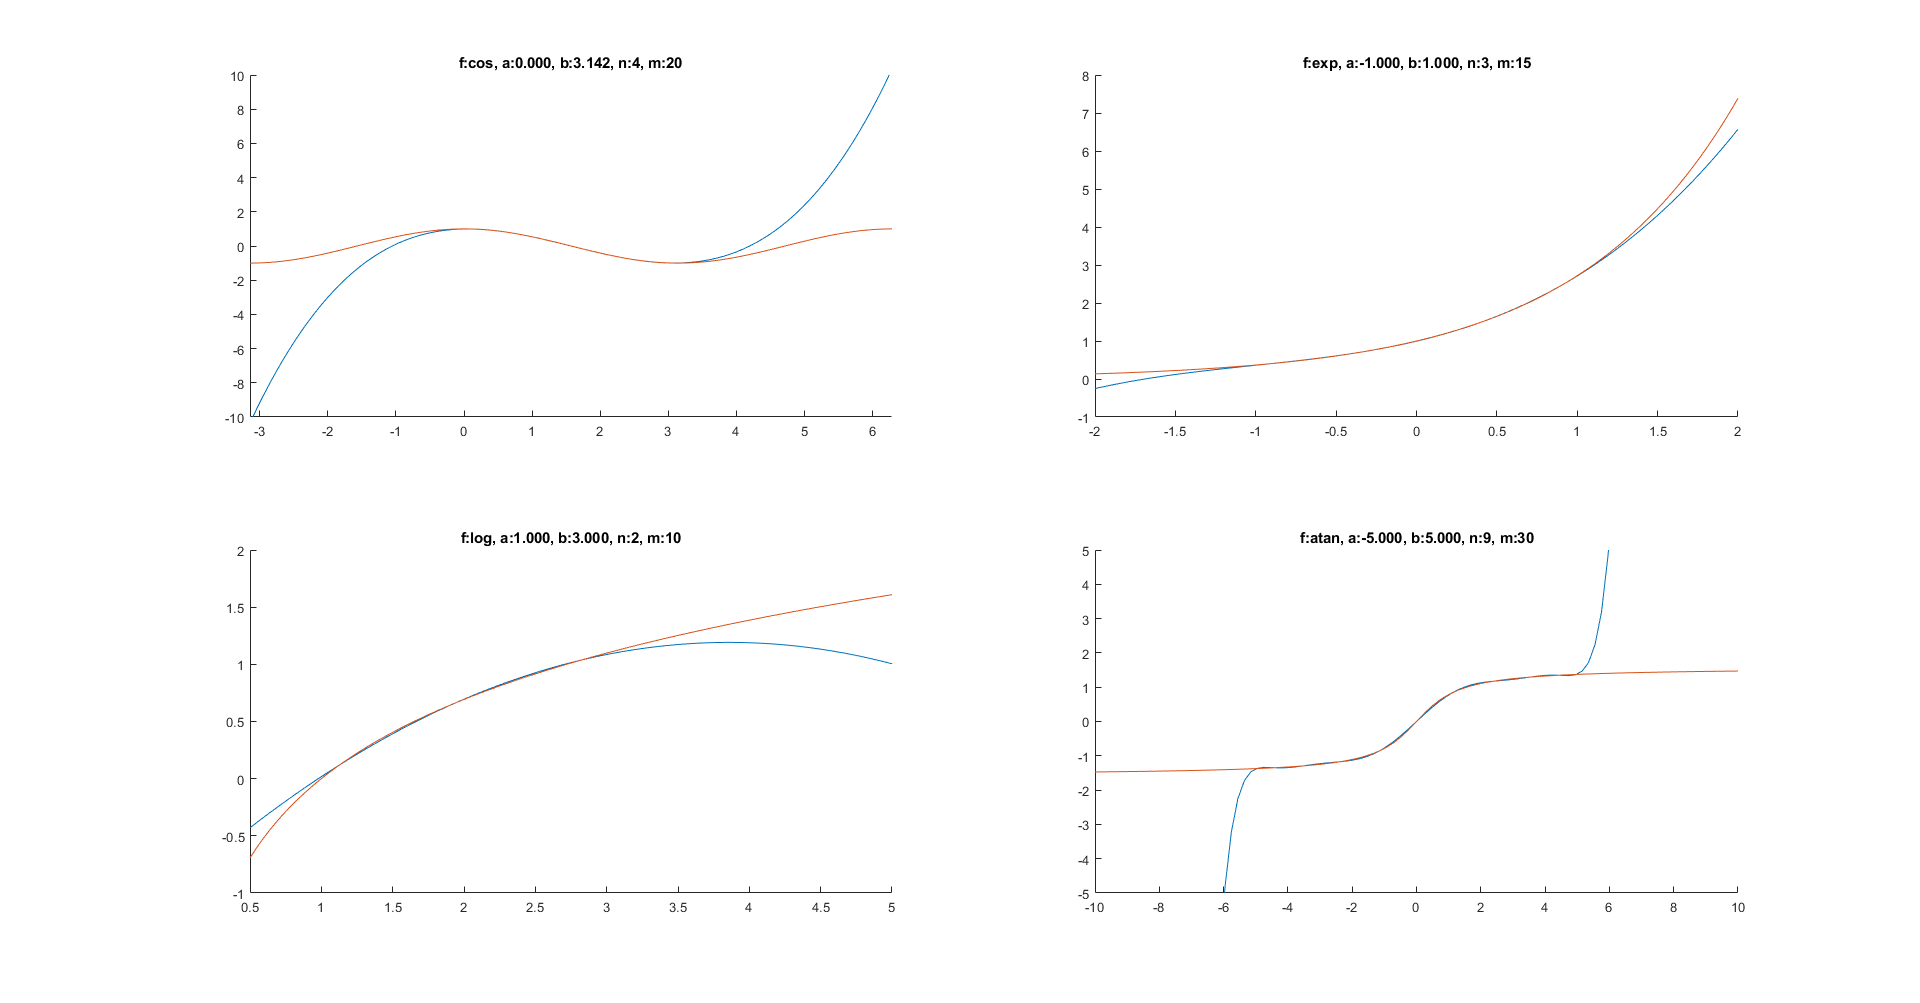
\includegraphics[width=\textwidth]{figures}
  \pgfplotstabletypeset[col sep=comma,
    columns={xi,pxi,cos xi, RelativeError},]{costable.csv}
  \pgfplotstabletypeset[col sep=comma,
    columns={xi,pxi,exp xi, RelativeError},]{exptable.csv}
  \pgfplotstabletypeset[col sep=comma,
    columns={xi,pxi,log xi, RelativeError},]{logtable.csv}
  \pgfplotstabletypeset[col sep=comma,
    columns={xi,pxi,atan xi, RelativeError},]{atantable.csv}
\end{enumerate}
\end{document}
